\ProvidesFile{rutitlepage.dtx}[2022/02/21 v3.0 Radboud University Titlepage]
\documentclass{ltxdoc}
\newcommand{\messagespace}{\text{$\mathcal{M}$}}
\newcommand{\messageinstance}{\text{$m$}}
\newcommand{\ciphertextspace}{\text{$\mathcal{C}$}}
\newcommand{\ciphertextinstance}{\text{$c$}}
\newcommand{\associateddataspace}{\text{$\mathcal{A}$}}
\newcommand{\associateddatainstance}{\text{$a$}}
\newcommand{\tagspace}{\text{$\mathcal{T}$}}
\newcommand{\taginstance}{\text{$t$}}
\newcommand{\keyspace}{\text{$\mathcal{K}$}}
\newcommand{\keyinstance}{\text{$k$}}
\newcommand{\noncespace}{\text{$\mathcal{N}$}}
\newcommand{\nonceinstance}{\text{$n$}}
\newcommand{\lockspace}{\text{$\mathcal{L}$}}
\newcommand{\lockinstance}{\text{$l$}}
\newcommand{\users}{\text{$N$}}
\newcommand{\user}{\text{$j$}}
\newcommand{\adversary}{\text{$A$}}
\newcommand{\sample}{\text{$\leftarrow$}}
\newcommand{\result}{\text{$\leftarrow$}}
\newcommand{\concatinate}{\text{$\|$}}

\newcommand{\advantage}[2]{\textbf{Adv}$_{\text{#1}}^{\text{#2}}$ }
\newcommand{\probabilityblock}[4]{\text{$|\text{Pr}[\text{#1}_{\text{#2}}^{\text{#3}}] - \text{Pr}[\text{#1}_{\text{#2}}^{\text{#4}}]|$}}

\newcommand{\pkc}{\text{Hybrid Encryption in a Multi-user Setting, revised}}
\newcommand{\gcrec}{\text{Generic Composition Reconsidered}}

\newcommand{\x}{\text{x}}
\usepackage{a4wide}
\usepackage{background}
\usepackage{float}
\usepackage{graphicx}
\usepackage{array}
\usepackage[utf8]{inputenc}
\usepackage{rutitlepage}
\usepackage{fancyhdr}
\usepackage[style=ieee]{biblatex}
\usepackage{cryptocode}
\addbibresource{cryptobib/crypto.bib}
\GetFileInfo{rutitlepage.dtx}

\pagestyle{fancy}
\fancyhf{}
\lhead{Bacholer Thesis}
\rhead{Page \thepage}

\backgroundsetup{
   scale=1,
   angle=0,
   opacity=1,
   color=black,
    contents={\begin{tikzpicture}[remember picture, overlay]
      \node at ([yshift=5.9 cm]current page.south)
            {
\includegraphics[width = \paperwidth]{template images/ruhuisstijl2017-en-169-redslide.pdf}} ;
     \end{tikzpicture}}
 }

\title{research proposal}
\author{stijnvandenput }
\date{20 May 2022}

\begin{document}
\maketitleru[
    layout=traditional,
    authors={Stijn Vandenput},
    authorstext={Author:},
    nextpagenr={-1},
    date={20/05/2022},
    institution={Radboud Honours Academy},
    others={Supervisor:}{Martijn Stam\\Bart Mennink},
    course={Bachelor Thesis},
    title={TBD}]

\section*{Abstract}

\pagenumbering{roman}
\newpage
\tableofcontents

\newpage
\pagenumbering{arabic}

\section{Introduction}
should consist of:
\begin{itemize}
	\item explaining the challenge
	\item my contribution
\end{itemize}

\section{Preliminaries}
should consist of:
\begin{itemize}
	\item recapping known definitions
	\item primitive definitions
\end{itemize}

\section{Existing AE/DEM notations in more detail}
should consist of:
\begin{itemize}
	\item the definition of the two paper, if possible already brought more toward one notation standard
\end{itemize}

\subsection{Existing notation from pkc}
\subsubsection{notation}
\messagespace is a message space, \keyspace is a finite key space, \tagspace is a tag space and \ciphertextspace is a ciphertext space. N is the number of users.
\subsubsection{used primitives}
\begin{itemize}
    \item ADEM: the ADEM exists of tuple (A.enc,A.dec), A.enc take a key K \keyspace, a tag t in \tagspace and a message m in \messagespace and outputs a ciphertext c in \ciphertextspace. A.dec takes a K \keyspace, a tag t in \tagspace and a ciphertext c in \ciphertextspace and outputs a message m in \messagespace or $\bot$ to indicate rejection. The correctness requirement is that for all K in \keyspace  and t in \tagspace and m in \messagespace we have A.dec(K,t,A.enc(K,t,m)) = m. The security of the ADEM is defined with \advantage{ADEM,A,N}{n-moit-ind} = \probabilityblock{N-MIOT-IND}{A,N}{0}{1}, defined by the following game:
    \begin{figure}[H]
        \centering
        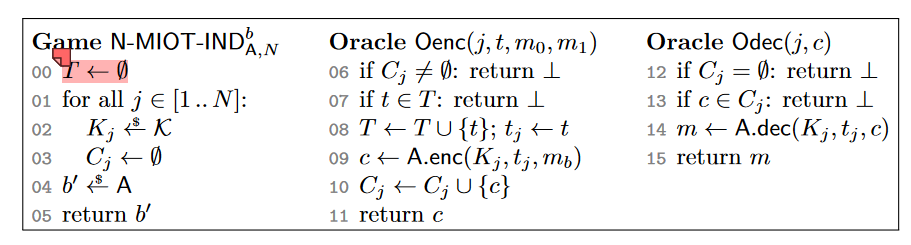
\includegraphics[scale = 0.5]{images/game adem.png}
    \end{figure}
    Where adversary A has access to oracles Oenc and Odec and the tags in line 9 and 14 are the same.
    
    \item AMAC: the AMAC exists of tuple (M.mac,M.vrf). M.mac takes a key K in \keyspace, a tag t in \tagspace, and a message m in \messagespace and outputs a ciphertext c in \ciphertextspace. M.vrf takes a key K in \keyspace, a tag t in \tagspace, a message m in \messagespace and a ciphertext c in \ciphertextspace and returns either true of false. The correctness requirement is that for all K in \keyspace, t in \tagspace and message in \messagespace and c in $[\text{M.mac(K,t,m)}]$ we have M.vrf(K,t,m,c)=true. The security of the AMAC is defined with \advantage{AMAC,A,N}{N-moit-uf} = Pr$[\text{N-MIOT-UF}_{\text{A,N}}]$, defined by the following game:
    \begin{figure}[H]
        \centering
        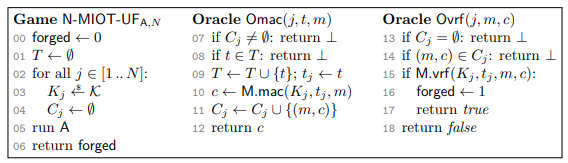
\includegraphics[scale = 0.5]{images/game amac.png}
    \end{figure}
    Where Adversary A can access oracles Omac and Ovrf and the tags in line 10 and 15 are the same.
\end{itemize}

\subsubsection{goal}
The goal is to make a scheme ADEM' from the ADEM and AMAC which has the same security of the ADEM, but is also secure against active attacks.

\subsubsection{Security model}
The security is defined by creating new A.enc' and A.dec' calls which are build using the calls the primitives provide us, and placing those in the ADEM game defined earlier:
\begin{figure}[H]
    \centering
    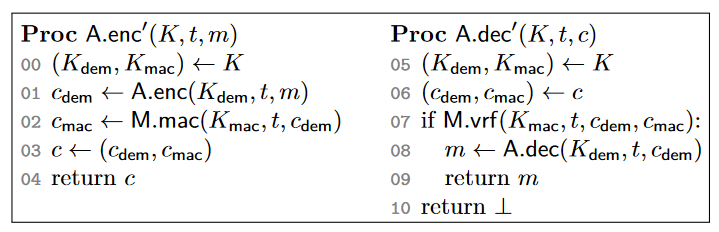
\includegraphics[scale = 0.5]{images/adem amac.png}
\end{figure}
The new advantage is \advantage{ADEM',A,N}{n-miot} $\leq$ 2\advantage{AMAC,B,N}{n-miot-uf} + \advantage{ADAM,C,N}{n-moit-ind}. Where the running time of B is at most that of A plus the time required to run N-many ADEM encapsulations and Qd-many ADEM decapsulations and the running time of C is the same as the running time of A. Additionally, B poses at most Qd-many Ovrf queries, and C poses no Odec query.

\subsection{Existing notation from generic composition reconsidered}
\subsubsection{notation}
\keyspace is a nonempty key space, \noncespace is a non-empty nonce space, \messagespace is a message space and \associateddataspace is the associated-data space. \messagespace (and \associateddataspace ? it's a bit ambiguous in the paper but I assume this part only applies to \messagespace) contain at least two strings, and if \messagespace and \associateddataspace contain a string of length x, they must contain all strings of length x.

\subsubsection{used primitives}
\begin{itemize}
    \item nE: A nonce-based E scheme is defined by triple (\keyspace,E,D). E is a deterministic encryption algorithm that takes three inputs (K,N,M) to a value C, the length of C only depends the length of K, N and M. When (K,N,M) is not in $\keyspacemathmode \times \noncespacemathmode \times \messagespacemathmode$, C will be $\bot$. D is the decryption algorithm that takes three inputs (K,N,C) to a value M. E and D are inverse of each other implying correctness (if E(K,N,M) $= C \neq \bot$, then D(K,N,C) = M) and tidiness (if D(K,N,C) $= M \neq \bot$, then E(K,N,M) = C). The security is defined as follows:\\ \fbox{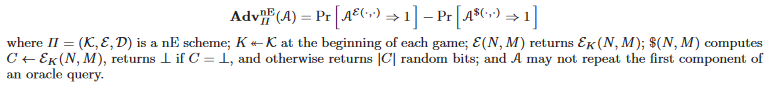
\includegraphics[scale = 0.8]{images/sec nE.png}}
    \item MAC: The MAC is a deterministic algorithm F that takes in a K in \keyspace and a string x and outputs either a n-bit length T or $\bot$. The domain of F is the set X such that F(K,x) $\neq \bot$. The security of F is defined by \advantage{F}{pfr} =\probabilityblock{A}{}{F}{p}. the game on the left selects a random K from \keyspace and provides oracle access to F(K,.) the game on the right selects a uniformly random function p from X to \{1,0\}$^n$ and provide oracle access to it. With each oracle, queries outside X return $\bot$
\end{itemize}

\subsubsection{goal}
The end goal is a nonce-based authenticated encryption scheme (\keyspace,E,D). E is a deterministic encryption algorithm that takes four inputs (K,N,A,M) to a value C, the length of C value only depends the length of K, N, A and M. When (K,N,A,M) is not in $\keyspacemathmode \times \noncespacemathmode \times \associateddataspacemathmode \times \messagespacemathmode$, C will be $\bot$. D is the decryption algorithm that takes four inputs (K,N,A,C) to a value M. E and D are inverse of each other implying correctness (if E(K,N,A,M) $= C \neq \bot$, then D(K,N,A,C) = M) and tidiness (if D(K,N,A,C) $= M \neq \bot$, then E(K,N,A,M) = C)
\subsubsection{Security model}
Security is defined as follows: \\ \fbox{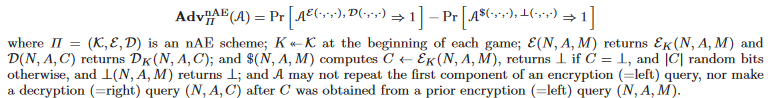
\includegraphics[scale = 0.88]{images/sec nAE.png}}\\
We define the scheme secure if there is a tight reduction from breaking the nAE-security of the scheme to breaking the nE-security and the PRF security of the underlying primitives.

\section{New Definition}
should consist of:
\begin{itemize}
	\item syntax of the primitive (input,output,correctness,tidiness, expected bounds)
	\item game based code
	\item explanation of the choices made
	\item formal comparison with other choices
\end{itemize}

\subsection{notation}
\keyspace is a nonempty key space, \noncespace is a non-empty nonce space and \messagespace is a message space. \messagespace contain at least two strings, and if it contain a string of length x, it must contain all strings of length x. N is the number of users.

\subsection{used primitives}
\begin{itemize}
    \item DEM: a DEM scheme is defined by tuple (E.enc,E.dec). E.enc is a deterministic encryption algorithm that takes three inputs (k,l,m) to a value c, the length of c only depends the length of k, l and m. When (k,l,m) is not in $\keyspacemathmode \times \lockspacemathmode \times \messagespacemathmode$, c will be $\bot$. E.dec is the decryption algorithm that takes three inputs (k,n,c) to a value m. E.enc and E.dec are inverse of each other implying correctness (if E.enc(k,l,m) $= c \neq \bot$, then E.dec(k,l,c) = m) and tidiness (if E.dec(k,N=l,c) $= m \neq \bot$, then E.enc(k,l,m) = c). The security is defined with the following game where \$.enc(k,l,m) calls c = E.enc(k,l,m) then outputs $\bot$ if c is $\bot$ or $\mid c \mid$ random bits otherwise and the advantage is calculated with \advantage{A,N}{DEM} = \probabilityblock{DEM}{A,N}{DEM}{\$}:
    \begin{figure}[H]
        \begin{pchstack}[boxed,center,space=0.5cm]
            \pseudocode[lnstart=-1,linenumbering,head={\textbf{Game} DEM$^E_{A,N}$ }]{
            L \leftarrow \emptyset\\
            \pcfor j \in [1..N]:\\
            \t K_j \leftarrow^\$ K\\
            b' \leftarrow A\\
            \pcreturn b'
            }
            \pseudocode[lnstart=4,linenumbering,head={\textbf{Oracle} Oenc(j,l,m)}]{
                \pcif T_j \neq \emptyset: \pcreturn \bot\\
                \pcif l \in L: \pcreturn \bot\\
                L \leftarrow L \cup \{l\}\\
                l_j = l\\
                c \leftarrow E.enc(K_j,l_j,m)\\
                \pcreturn c
            }
        \end{pchstack}
    \caption{DEM game where E is either the DEM or a random function \$, adversary A has access to Oenc}
    \end{figure} 
    
    \item MAC: The MAC is a deterministic algorithm M.mac that takes in a fixed length k in \keyspace, a fixed length l in \lockspace and a variable length message m in \messagespace and outputs either a n-bit length tag or $\bot$. The domain of M.mac is the set X such that M.mac(k,l,m) $\neq \bot$. The security of F is defined by the following security game where \$.mac(k,l,m) calls t = M.mac(k,l,m) then outputs $\bot$ if t is $\bot$ or $\mid t \mid$ random bits otherwise and the advantage is calculated with \advantage{A,N}{MAC} = \probabilityblock{MAC}{A,N}{MAC}{\$}:
    \begin{figure}[H]
        \begin{pchstack}[boxed,center,space=0.5cm]
            \pseudocode[lnstart=-1,linenumbering,head={\textbf{Game} MAC$^M_{A,N}$ }]{
            L \leftarrow \emptyset\\
            \pcfor j \in [1..N]:\\
            \t K_j \leftarrow^\$ K\\
            b' \leftarrow A\\
            \pcreturn b'
            }
            \pseudocode[lnstart=4,linenumbering,head={\textbf{Oracle} Omac(j,l,m)}]{
                \pcif T_j \neq \emptyset: \pcreturn \bot\\
                \pcif l \in L: \pcreturn \bot\\
                L \leftarrow L \cup \{l\}\\
                l_j = l\\
                t \leftarrow M.mac(K_j,l_j,m)\\
                \pcreturn t
            }
        \end{pchstack}
    \caption{MAC game where M is either the MAC or a random function \$, adversary A has access to Omac}
    \end{figure}
\end{itemize}

\subsection{goal}
The end goal is to build a Authenticated Encryption scheme (EA) secure against active attacks from the underlying primitives. The AE scheme is defined by tuple (AE.enc,AE.dec). AE.enc is a deterministic encryption algorithm that takes three inputs (k,l,m) to a value c, the length of c only depends the length of k, l and m. When (k,l,m) is not in $\keyspacemathmode \times \lockspacemathmode \times \messagespacemathmode$, c will be $\bot$. AE.dec is the decryption algorithm that takes three inputs (k,n,c) to a value m. AE.enc and E.dec are inverse of each other implying correctness (if AE.enc(k,l,m) $= c \neq \bot$, then AE.dec(k,l,c) = m) and tidiness (if AE.dec(k,N=l,c) $= m \neq \bot$, then AE.enc(k,l,m) = c).

\subsection{Security model}
The security is defined by the following security game where \$.enc(k,l,m) calls c = AE.enc(k,l,m) then outputs $\bot$ if c is $\bot$ or $\mid c \mid$ random bits otherwise. \$.dec(k,l,c) always returns $\bot$ and the advantage is calculated with \advantage{A,N}{AE} = \probabilityblock{AE}{A,N}{AE}{\$}:
\begin{figure}[H]
    \begin{pchstack}[boxed,center,space=0.5cm]
        \pseudocode[lnstart=-1,linenumbering,head={\textbf{Game} AE$^{AE}_{A,N}$ }]{
        L \leftarrow \emptyset\\
        \pcfor j \in [1..N]:\\
        \t K_j \leftarrow^\$ K\\
        \t C_j \leftarrow \emptyset\\
        b' \leftarrow A\\
        \pcreturn b'
        }
        \pseudocode[lnstart=5,linenumbering,head={\textbf{Oracle} Oenc(j,l,m)}]{
            \pcif T_j \neq \emptyset: \pcreturn \bot\\
            \pcif l \in L: \pcreturn \bot\\
            L \leftarrow L \cup \{l\}\\
            l_j = l\\
            c \leftarrow AE.enc(K_j,l_j,m)\\
            C_j \leftarrow C_j \cup c\\
            \pcreturn t
        }
        \pseudocode[lnstart=12,linenumbering,head={\textbf{Oracle} Odec(j,m)}]{
            \pcif c_j \neq \emptyset: \pcreturn \bot\\
            \pcif c \in C_j: \pcreturn \bot\\
            m \leftarrow AE.dec(K_j,L_j,c)\\
            \pcreturn m
        }
    \end{pchstack}
\caption{AE game, where AE is either the AE scheme build from the MAC and DEM or a random function \$, adversary A has access to Oenc and Odec}
\end{figure}
The scheme is considered secure when there is a tight reduction from breaking the AE-security of the scheme to breaking the defined security of the underlying primitives.

\subsection(choices made)

\section{Constructions}
should consist of:
\begin{itemize}
	\item how to construct the new primitive from old primitives
	\item security bounds + proof
	\item comparison with existing alternatives
\end{itemize}

\noindent The AE schemes should be constructed from the DEM and the MAC. Following General Composition reconsidered, three ways to construct this AE are of interest, namely the ones following from the N1, N2 and N3 scheme. One thing to keep in mind with this that these schemes would originally use associated data. For now we can discard this but it is not proven that the same security results would also follow from this case without associated data. Down here the initial schemes can be found, followed by the AE.enc and AE.dec calls that can we construct following these schemes.
\begin{figure}[H]
    \centering
    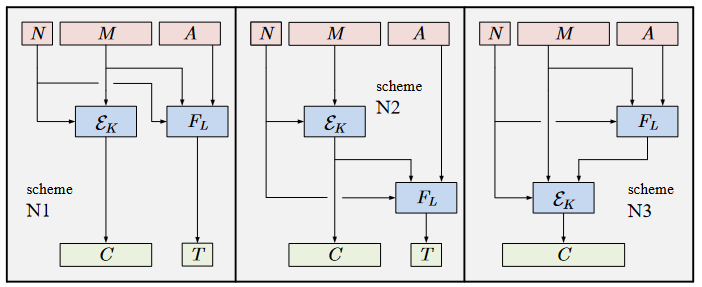
\includegraphics[scale = 0.7]{images/N games.png}
\caption{Original N schemes from Generic Composition reconsidered}
\end{figure}

\begin{figure}[H]
    \begin{pchstack}[boxed,center,space=0.5cm]
        \pseudocode[lnstart=-1,linenumbering,head={AE.enc(k,l,m)}]{
            (k1,k2) \leftarrow k \\
            c' = E.enc(k1,l,m) \\
            t = M.mac(k2,l,m) \\
            c = (c',t)\\
            \pcreturn c
        }
        \pseudocode[lnstart=4,linenumbering,head={AE.dec(k,l,c)}]{
            (k1,k2) \leftarrow k \\
            (c',t) \leftarrow c \\
            m = E.dec(k1,l,c') \\
            t' = M.mac(k2,l,m) \\
            \pcif t = t' : \pcreturn m \\
            \pcelse : \pcreturn \bot
        }
    \end{pchstack}
\caption{Calls based on N1}
\end{figure}

\begin{figure}[H]
    \begin{pchstack}[boxed,center,space=0.5cm]
        \pseudocode[lnstart=-1,linenumbering,head={AE.enc(k,l,m)}]{
            (k1,k2) \leftarrow k\\
            c' = E.enc(k1,l,m)\\
            t = M.mac(k2,l,c')\\
            c = (c',t)\\
            \pcreturn c
        }
        \pseudocode[lnstart=4,linenumbering,head={AE.dec(k,l,c)}]{
            (k1,k2) \leftarrow k\\
            (c',t) \leftarrow c\\
            m = E.dec(k1,l,c')\\
            t' = M.mac(k2,l,c')\\
            \pcif t = t' : \pcreturn m \\
            \pcelse : \pcreturn \bot
        }
    \end{pchstack}
\caption{Calls based on N2}
\end{figure}

\begin{figure}[H]
    \begin{pchstack}[boxed,center,space=0.5cm]
        \pseudocode[lnstart=-1,linenumbering,head={AE.enc(k,l,m)}]{
            (k1,k2) \leftarrow k\\
            t = M.mac(k2,l,m)\\
            m' = m || t\\
            c = E.enc(k1,l,m')\\
            \pcreturn c
        }
        \pseudocode[lnstart=4,linenumbering,head={AE.dec(k,l,c)}]{
            (k1,k2) \leftarrow k\\
            m' = E.dec(k1,l,c)\\
            (m,t) \leftarrow m'\\
            t' = M.mac(k2,l,m)\\
            \pcif t = t' : \pcreturn m \\
            \pcelse : \pcreturn \bot
        }
    \end{pchstack}
\caption{Calls based on N3}
\end{figure}

\section{Use cases}
should consist of:
\begin{itemize}
	\item possible use cases
\end{itemize}

\section{Related Work}
\textbf{Location not final yet}

\section{Conclusion}

\newpage
\printbibliography[heading=bibintoc,title={References}]
\section{Appendix}

\end{document}

\NeedsTeXFormat{LaTeX2e}
\ProvidesPackage{rutitlepage}[2022/02/21 Mart Lubbers]
\RequirePackage{geometry,graphicx,ifpdf,keyval,iflang}
\def\@rutitleauthors{\@author}
\def\@rutitleauthorstext{Aut\IfLanguageName{dutch}{eu}{ho}r:}
\def\@rutitledate{\@date}
\def\@rutitleinst{Radboud Universit\IfLanguageName{dutch}{eit}{y} Nijmegen}
\def\@rutitletitle{\@title}
\def\@rutitlelayout{twentytwo}
\newif\if@rutitlecolour\@rutitlecolourfalse
\define@key{maketitleru}{authors}{\def\@rutitleauthors{#1}}
\define@key{maketitleru}{authorstext}{\def\@rutitleauthorstext{#1}}
\define@key{maketitleru}{colour}[true]{\@rutitlecolourtrue}
\define@key{maketitleru}{course}{\def\@rutitlecourse{#1}}
\define@key{maketitleru}{date}{\def\@rutitledate{#1}}
\define@key{maketitleru}{institution}{\def\@rutitleinst{#1}}
\define@key{maketitleru}{layout}{\def\@rutitlelayout{#1}}
\define@key{maketitleru}{nextpagenr}{\def\@rutitlenextpagenr{#1}}
\define@key{maketitleru}{others}{\def\@rutitleothers{#1}}
\define@key{maketitleru}{subtitle}{\def\@rutitlesubtitle{#1}}
\define@key{maketitleru}{title}{\def\@rutitletitle{#1}}
\newcommand*{\rutitlepage@printothers}[2]{\textit{#1}\\#2}
\newcommand*{\rutitlepage@sepothers}{\\[\baselineskip]}
\newcommand*{\rutitlepage@others}[2]{%
	\rutitlepage@printothers{#1}{#2}%
	\kernel@ifnextchar,{\rutitlepage@sepothers\rutitlepage@otherslist@}\relax}
\newcommand*{\rutitlepage@otherslist}[1]{%
	\expandafter\rutitlepage@others#1}
\def\rutitlepage@otherslist@,#1{\rutitlepage@otherslist{{#1}}}
\newcommand{\rutitle@layout@twentytwo}[0]{
	\newgeometry{left=25mm,top=25mm,right=15mm,bottom=10mm,hmarginratio=1:1}
	\begin{titlepage}%
		\null\vfill%
		\parindent0pt
		\ifdefined\@rutitlecourse\textsc{\LARGE\@rutitlecourse}\\[1.5cm]\fi
		{\Huge\bfseries\@rutitletitle}%
		\ifdefined\@rutitlesubtitle{\\[2\baselineskip]\large\itshape\@rutitlesubtitle\/}\fi\\[4\baselineskip]
		{\Large\scshape\@rutitleauthors}\\[\baselineskip]
		{\large\@rutitledate}
		\vfill

		\ifdefined\@rutitleothers\rutitlepage@otherslist\@rutitleothers\fi
		\vfill

		\hfill
		\ifpdf\includegraphics[width=80mm]{rutitlepage-logo-\IfLanguageName{dutch}{nl-}{}\if@rutitlecolour cmyk\else bw\fi.pdf}\\
		\else\includegraphics[width=80mm]{rutitlepage-logo-\IfLanguageName{dutch}{nl-}{}\if@rutitlecolour cmyk\else bw\fi.eps}\\
		\fi
	\end{titlepage}
	\restoregeometry%
}
\newcommand{\rutitle@layout@seventeen}[0]{
	\newgeometry{left=25mm,top=25mm,right=15mm,bottom=10mm,hmarginratio=1:1}
	\begin{titlepage}%
		\null\vfill%
		\parindent0pt
		{\Huge\bfseries\@rutitletitle}%
		\ifdefined\@rutitlesubtitle{\\[2\baselineskip]\large\itshape\@rutitlesubtitle\/}\fi\\[4\baselineskip]
		{\Large\scshape\@rutitleauthors}\\[\baselineskip]
		{\large\@rutitledate}
		\vfill

		\ifdefined\@rutitleothers\rutitlepage@otherslist\@rutitleothers\fi
		\vfill

		\hfill
		\ifpdf\includegraphics[width=80mm]{rutitlepage-logo-\IfLanguageName{dutch}{nl-}{}\if@rutitlecolour cmyk\else bw\fi.pdf}\\
		\else\includegraphics[width=80mm]{rutitlepage-logo-\IfLanguageName{dutch}{nl-}{}\if@rutitlecolour cmyk\else bw\fi.eps}\\
		\fi
	\end{titlepage}
	\restoregeometry%
}
\newcommand{\rutitle@layout@traditional}[0]{
	\newgeometry{hmarginratio=1:1}
	\begin{titlepage}
		\begin{center}
			\ifdefined\@rutitlecourse\textsc{\LARGE\@rutitlecourse}\\[1.5cm]\fi
			\ifpdf\includegraphics[height=150pt]{rutitlepage-logo.pdf}\\
			\else\includegraphics[height=150pt]{rutitlepage-logo.eps}\\
			\fi
			\vspace{0.4cm}
			\textsc{\Large\@rutitleinst}\\[1cm]
			\hrule
			\vspace{0.4cm}
			\textbf{\large\@rutitletitle}\\[0.4cm]
			\hrule
			\ifdefined\@rutitlesubtitle
				\vspace{0.4cm}
				\textit{\@rutitlesubtitle}\\[1cm]
			\else
				\vspace{2cm}
			\fi
			\begin{minipage}[t]{0.45\textwidth}
				\begin{flushleft}\large
					\textit{\@rutitleauthorstext}\\
					\@rutitleauthors{}
				\end{flushleft}
			\end{minipage}
			\begin{minipage}[t]{0.45\textwidth}
				\begin{flushright}\large
					\ifdefined\@rutitleothers
					\renewcommand{\rutitlepage@printothers}[2]{\textit{##1}\\##2}
					\renewcommand{\rutitlepage@sepothers}[0]{

						\vspace{8mm}}
					\rutitlepage@otherslist\@rutitleothers
					\fi
				\end{flushright}
			\end{minipage}
			\vfill
			{\large\@rutitledate}
		\end{center}
	\end{titlepage}
	\restoregeometry%
}
\newcommand{\maketitleru}[1][]{
	\setkeys{maketitleru}{#1}
	\ifcsname%
		rutitle@layout@\@rutitlelayout\endcsname
		\expandafter\csname rutitle@layout@\@rutitlelayout\endcsname
	\else
		\PackageError{rutitlepage}
			{Unknown layout `\@rutitlelayout'.}
			{The `layout' key of \maketitleru\space contained an unknown layout.\MessageBreak{}
			 Check the package documentation for the possible layouts.}
	\fi
	\ifdefined\@rutitlenextpagenr\setcounter{page}{\@rutitlenextpagenr}\fi%
}